% !TeX encoding = UTF-8
% !TeX spellcheck = fr_FR
% !TeX root = mythesis.tex
\newcommand{\adag}[1]{\hat{a}_{#1}^\dagger}
\newcommand{\aop}[1]{\hat{a}_{#1\vphantom{\dagger}}}

\chapter{ Theory: background} \label{chap:theory}
This chapter will cover the elementary concepts required to describe an membrane based optomechanical system in a quantum regime. We will first recall basics on optical field quantization as well describing coherent and squeezed light field, to then turn to the more specific frequency dependent squeezed light field. Secondly, we will cover the mathematical description of a mechanical resonator interacting with a generic coherent optical field, highlighting the differences with the seminal optomechanical system of a mirror on a spring. Finally, we will derive the equations of motions of a membrane based optomechanical system with frequency dependent squeezed optical fields. 

\section{Quantum Optics Concepts}
\subsection{Quantum Description of Light}
We introduce briefly field quantization concepts needed to describe monochromatic field propagation and measurements.
key words : eigenmodes of the field, quantization, annihilation operators, quadratures, phase space, displacement operators, squeezing operators, coherent states, generic squeezed states,


\subsection*{Quantised Electromagnetic Field}
% \the\textwidth

We consider the quantised electromagnetic field in volume $V$. The electric field operator can be expressed in the Heisenberg picture as:
\begin{equation}
\hat{\mathbf{E}}(\mathbf{r}, t) = i \sum_{ \ell} \mathcal{E}_l \left[\hat{a}_{\ell}^{\vphantom{dagger}}\mathbf{f}_{\ell}(\mathbf{r})e^{-i\omega_{\ell}t} - \hat{a}_{\ell}^\dagger \mathbf{f}_{\ell}^*(\mathbf{r}) e^{i\omega_{\ell}t}\right]
\end{equation}
where $\mathcal{E}_l = \sqrt{\frac{\hbar \omega_l}{2 \varepsilon_0 V}}$ is the field per photon in mode $\ell$ with $\hbar$ the reduced Planck constant, $\omega_\ell$ the angular frequency of mode $\ell$ and $\varepsilon_0$ the vacuum permittivity, $\mathbf{f}_{\ell}(\mathbf{r})$ are spatial mode functions satisfying orthonormality, and ($\hat{a}_{\ell}^{\vphantom{\dagger}}$, $\hat{a}_{\ell}^{\dagger}$) are the time dependent annihilation and creation operators associated with each mode $\ell$ satisfying the canonical commutation relations
\[
[\hat{a}_{\ell}^{\vphantom{\dagger}}, \hat{a}_{\ell'}^\dagger] = \delta_{\ell \ell'} , \quad
[\hat{a}_{\ell}^{\vphantom{\dagger}}, \hat{a}_{\ell'}^{\vphantom{\dagger}} ] = 0, \quad [\hat{a}_{\ell}^\dagger , \hat{a}_{\ell'}^\dagger ] = 0  
\]
\subsection*{Fock states}
In this description of the optical field, each mode $\ell$ is modeled as a quantum harmonic oscillator with a discrete set of energy eigenstates known as \textit{Fock states} or number states, denoted $\ket{n_\ell}$. These states form an orthonormal basis and satisfy $\hat{n}_{\ell} \ket{n_\ell} = n_\ell \ket{n_\ell}$, where $\hat{n}_{\ell}$ is the number operator defined by
\[
\hat{n}_{\ell} = \hat{a}_{\ell}^\dagger \hat{a}^{\vphantom{\dagger}}_{\ell}.
\]
The action of the creation and annihilation operators on these states is given by
\[
\hat{a}^{\vphantom{\dagger}}_{\ell} \ket{n_\ell} = \sqrt{n_\ell} \ket{n_\ell - 1}, \quad
\hat{a}_{\ell}^\dagger \ket{n_\ell} = \sqrt{n_\ell + 1} \ket{n_\ell + 1}.
\]
They allow transitions between Fock states by lowering or raising the photon number in mode $\ell$ by one unit. The vacuum state $\ket{0_\ell}$ is annihilated by $\hat{a}^{\vphantom{\dagger}}_{\ell}$, satisfying $\hat{a}^{\vphantom{\dagger}}_{\ell} \ket{0_\ell} = 0$. Thus, the Hamiltonian for the electromagnetic field becomes a sum of harmonic oscillator energies:
\begin{equation}
\hat{H} = \sum_\ell \hbar \omega_{\ell} \left( \hat{n}_\ell + \frac{1}{2} \right)
\end{equation}
\color{red} \subsection*{Quasi monochromatic fields and slow variations} \color{black}
finite linewidth laser fields, slow variations of the eigenvalue of operator $\hat{a}$ compared to the optical frequency, slow variations imply spectral decomposition of the field, make $\hat{a}$ time dependent 
\color{red} \subsection*{Linearization of the optical field, mean field and fluctuations} \color{black} 
We will often consider a single spatial mode of the electromagnetic field, as well as a strong optical field translating to $\hat{a}(t)=\bar{\alpha} + \delta \hat{a}(t)$.  linearizing such that the field simplifies to  
\begin{equation}
\hat{\mathbf{E}}(\mathbf{r}, t) = i \mathcal{E} \left(\hat{a}^{\vphantom{dagger}}(t)\mathbf{f}(\mathbf{r})e^{-i\omega_{\ell}t} - \hat{a}^\dagger(t) \mathbf{f}^*(\mathbf{r})e^{i\omega_{\ell}t} \right)
\end{equation}
where we drop the $\ell$ subscript to simplify the notation. The field Hamiltonian then reduces to a single harmonic oscillator Hamiltonian $\hat{H} = \hbar \omega \hat{a}^{\dagger} \hat{a}^{\vphantom{dagger}}$ where we also drop the constant energy offset $\hbar \omega/2$.\\

\noindent\textbf{Remarks:}



\color{red} \subsection*{Coherent and squeezed states }



\color{black}
\subsection*{Quadrature Operators}

To describe the phase space properties of a field mode, we define the Hermitian quadrature operators $X_{1,l}$ and $X_{2,l}$ as
\begin{equation}
  \begin{split}
    \hat{X}_{1,l} &= \hat{a}^{\vphantom{\dagger}}_{\ell} + \hat{a}_{\ell}^\dagger  \\
    \hat{X}_{2,l} &= \hat{a}^{\vphantom{\dagger}}_{\ell} - \hat{a}_{\ell}^\dagger
  \end{split}
\end{equation}
More generally we can define arbitrary quadrature operators as 
\begin{align}
  \hat{X}_{\theta,l} &= e^{i\theta}\hat{a}_{\ell}+ e^{-i\theta}\hat{a}_{\ell}^{\dagger} \notag \\ 
  & = \cos \theta \hat{X}_{1,l} + \sin \theta \hat{X}_{2,l}
\end{align}
where we notice that $\hat{X}_{1,l} = \hat{X}_{\theta=0\vphantom{\pi/2},l}$ and $\hat{X}_{1,l} = \hat{X}_{\theta=\pi/2,l}$. These are Hermitian operators corresponding to measurable observables and satisfy the commutation relation
\begin{equation}
[X_{\theta \vphantom{\pi/2},l}, X_{\theta+\pi/2,l}] = 2i
\end{equation}

\subsection*{Uncertainty Principle and Quantum Noise}

For two generic Hermitian operators $\hat{A}$ and $\hat{B}$, the Heisenberg uncertainty principle reads as 
\begin{equation}
  \Delta \hat{A}\Delta \hat{B} > \frac{1}{2} |[\hat{A}, \hat{B}]|
\end{equation}
where we defines $\Delta \hat{A}=\sqrt{|\langle \hat{A}^2\rangle - \langle \hat{A} \rangle^2|}$. This defines the minimum amount of quantum noise (vacuum fluctuations) in the electromagnetic field.
Applying this equation to the quadratures defined above we get 
\begin{equation}
   \begin{split}
    \Delta \hat{X}_{1,l} \Delta \hat{X}_{2,l} &> 1 \\
    \Delta X_{\theta \vphantom{\pi/2},l} \Delta X_{\theta \vphantom{\pi/2},l} &> 1
   \end{split}
\end{equation}
\subsection*{Coherent States}


\begin{figure}
\centering
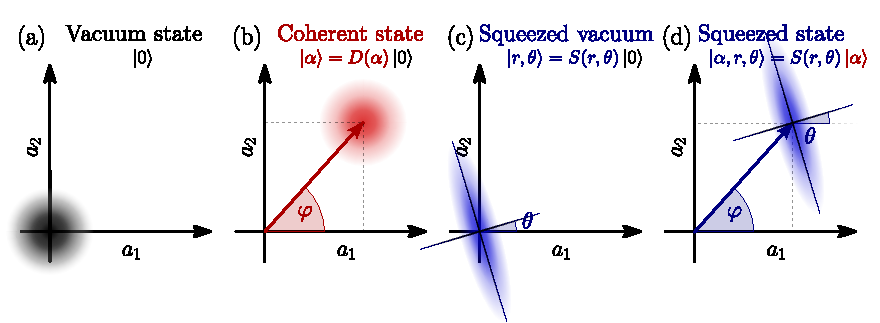
\includegraphics[width=\textwidth]{./chap2/fig/quantumstates (2).pdf}
\caption{Phase-space representations of quantum states and transformations.
(a) Wigner function of the vacuum state: a circular Gaussian centered at the origin, representing equal quantum fluctuations in both quadratures $X_1$ and $X_2$.
(b) Wigner function of a coherent state: a displaced circular Gaussian, showing a shift in phase space along an angle $\varphi$ with unchanged, isotropic noise.
(c) Wigner function of a squeezed vacuum state: an elliptical Gaussian centered at the origin, with reduced noise along a rotated quadrature $X_\theta$ and increased noise in the orthogonal direction.
(d) Wigner function of a displaced squeezed state: an ellipse shifted away from the origin, combining anisotropic fluctuations and a nonzero mean amplitude. The displacement angle $\varphi$ and squeezing angle $\theta$ are independent.} 
\end{figure}

\begin{figure}
\centering
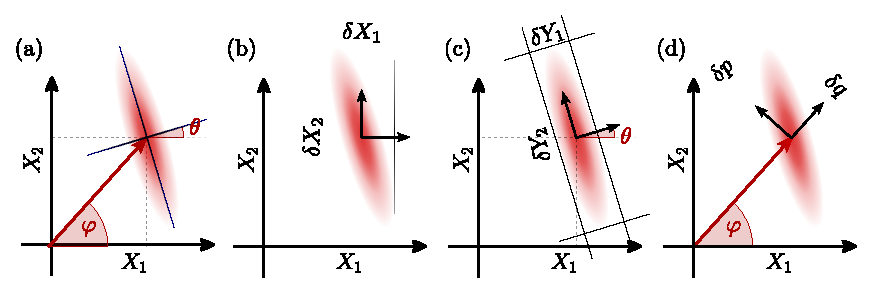
\includegraphics[width=\textwidth]{./chap2/fig/quadratures_phasespace.pdf}
\caption{Phase-space representations of quantum states and transformations.
(a) Wigner function of the vacuum state: a circular Gaussian centered at the origin, representing equal quantum fluctuations in both quadratures $X_1$ and $X_2$.
(b) Wigner function of a coherent state: a displaced circular Gaussian, showing a shift in phase space along an angle $\varphi$ with unchanged, isotropic noise.
(c) Wigner function of a squeezed vacuum state: an elliptical Gaussian centered at the origin, with reduced noise along a rotated quadrature $X_\theta$ and increased noise in the orthogonal direction.
(d) Wigner function of a displaced squeezed state: an ellipse shifted away from the origin, combining anisotropic fluctuations and a nonzero mean amplitude. The displacement angle $\varphi$ and squeezing angle $\theta$ are independent.} 
\end{figure}


Coherent states $|\alpha_{\omega,\ell}\rangle$ are eigenstates of the annihilation operator:
\begin{equation}
\hat{a}_{\omega,\ell}|\alpha_{\omega,\ell}\rangle = \alpha_{\omega,\ell}|\alpha_{\omega,\ell}\rangle
\end{equation}
They can be generated by displacing the vacuum:
\begin{equation}
|\alpha_{\omega,\ell}\rangle = \hat{D}(\alpha_{\omega,\ell})|0\rangle, \quad \hat{D}(\alpha) = \exp(\alpha \hat{a}^\dagger - \alpha^* \hat{a})
\end{equation}
They exhibit:
\begin{itemize}
  \item Minimum uncertainty: $\Delta q = \Delta p = 1/\sqrt{2}$
  \item Classical-like dynamics
  \item Poissonian photon statistics
\end{itemize}

\subsection*{Squeezed States}

Squeezed states reduce the variance of one quadrature below vacuum level:
\begin{align}
|\xi_{\omega,\ell}\rangle &= \hat{S}(\xi_{\omega,\ell}) |0\rangle \\
\hat{S}(\xi) &= \exp\left[\frac{1}{2}(\xi^* \hat{a}^2 - \xi \hat{a}^{\dagger 2})\right], \quad \xi = r e^{i\phi}
\end{align}
For phase quadrature squeezing ($\phi = 0$):
\begin{equation}
\Delta q_{\omega,\ell} = e^{-r}/\sqrt{2}, \quad \Delta p_{\omega,\ell} = e^{r}/\sqrt{2}
\end{equation}
Squeezed light is a key resource for precision metrology and quantum information.


\vspace{1em}
This concludes our introduction to the quantum description of light, setting the stage for modelling interactions between quantum optical fields and mechanical resonators.

\subsection{\textcolor{red}{Optical Field Modulations}}
\subsubsection*{Linearization of the Electric Field and Modulation Sidebands}

We consider a single optical mode with a strong coherent drive. The annihilation operator is linearized as:
\begin{equation}
    \hat{a}(t) \to \bar{\alpha}(t) + \delta \hat{a}(t)
\end{equation}
where $\bar{\alpha}(t) \in \mathbb{C}$ is the classical coherent amplitude and $\delta \hat{a}(t)$ captures quantum fluctuations.

The classical part of the electric field is then:
\begin{equation}
    \mathbf{E}_{\text{cl}}(\mathbf{r}, t) = i \sqrt{\frac{\hbar \omega}{2 \varepsilon_0}} \left[
    \mathbf{f}(\mathbf{r})\, \bar{\alpha}(t)\, e^{-i \omega t}
    - \mathbf{f}^*(\mathbf{r})\, \bar{\alpha}^*(t)\, e^{i \omega t}
    \right]
\end{equation}

We now consider two types of sinusoidal modulation at frequency $\Omega$:

\subsubsection*{Amplitude Modulation (AM)}

Let the coherent amplitude be modulated in amplitude:
\begin{equation}
    \bar{\alpha}(t) = \bar{\alpha}_0 \left(1 + \epsilon_a \cos(\Omega t)\right)
    = \bar{\alpha}_0 \left(1 + \frac{\epsilon_a}{2} e^{i\Omega t} + \frac{\epsilon_a}{2} e^{-i\Omega t} \right)
\end{equation}
with $\epsilon_a \ll 1$. The conjugate is:
\begin{equation}
    \bar{\alpha}^*(t) = \bar{\alpha}_0^* \left(1 + \frac{\epsilon_a}{2} e^{i\Omega t} + \frac{\epsilon_a}{2} e^{-i\Omega t} \right)
\end{equation}

Substituting into the field expression:
\begin{align}
    \mathbf{E}_{\text{cl}}^{\text{(AM)}}(\mathbf{r}, t) =
    i \sqrt{\frac{\hbar \omega}{2 \varepsilon_0}} \Big[
    &\mathbf{f}(\mathbf{r})\, \bar{\alpha}_0 \left( e^{-i\omega t} + \frac{\epsilon_a}{2} e^{-i(\omega - \Omega)t} + \frac{\epsilon_a}{2} e^{-i(\omega + \Omega)t} \right) \nonumber \\
    - &\mathbf{f}^*(\mathbf{r})\, \bar{\alpha}_0^* \left( e^{i\omega t} + \frac{\epsilon_a}{2} e^{i(\omega - \Omega)t} + \frac{\epsilon_a}{2} e^{i(\omega + \Omega)t} \right)
    \Big]
\end{align}

\subsubsection*{Phase Modulation (PM)}

Now consider phase modulation of the coherent amplitude:
\begin{equation}
    \bar{\alpha}(t) = \bar{\alpha}_0 e^{i \epsilon_\phi \cos(\Omega t)}
    \approx \bar{\alpha}_0 \left(1 + i \epsilon_\phi \cos(\Omega t)\right)
    = \bar{\alpha}_0 \left(1 + \frac{i \epsilon_\phi}{2} e^{i\Omega t} + \frac{i \epsilon_\phi}{2} e^{-i\Omega t} \right)
\end{equation}
and
\begin{equation}
    \bar{\alpha}^*(t) \approx \bar{\alpha}_0^* \left(1 - \frac{i \epsilon_\phi}{2} e^{i\Omega t} - \frac{i \epsilon_\phi}{2} e^{-i\Omega t} \right)
\end{equation}

Substituting into the field:
\begin{align}
    \mathbf{E}_{\text{cl}}^{\text{(PM)}}(\mathbf{r}, t) =
    i \sqrt{\frac{\hbar \omega}{2 \varepsilon_0}} \Big[
    &\mathbf{f}(\mathbf{r})\, \bar{\alpha}_0 \left( e^{-i\omega t} + \frac{i \epsilon_\phi}{2} e^{-i(\omega - \Omega)t} + \frac{i \epsilon_\phi}{2} e^{-i(\omega + \Omega)t} \right) \nonumber \\
    - &\mathbf{f}^*(\mathbf{r})\, \bar{\alpha}_0^* \left( e^{i\omega t} - \frac{i \epsilon_\phi}{2} e^{i(\omega - \Omega)t} - \frac{i \epsilon_\phi}{2} e^{i(\omega + \Omega)t} \right)
    \Big]
\end{align}

\subsection*{Interpretation}

In both cases, the field contains a carrier at frequency $\omega$ and two sidebands at $\omega \pm \Omega$. Amplitude modulation results in sidebands that are in phase with the carrier, while phase modulation produces sidebands with a $\pm \pi/2$ phase shift relative to the carrier.

\subsection{Quantum Noise and Uncertainty}
\subsection{Sideband Representation}
\hspace{1pt}

\section{Optical Cavities : Basics}
\subsection{Cavity types and Resonance Conditions}
\subsection{Spatial and Longitudinal Modes}
\subsection{Static and Dynamical effects}
\hspace{1pt}

\section{\texorpdfstring{\color{red}Optical Cavities : Three Mirror Cavities}{Optical Cavities : Three Mirror Cavities}}
\subsection{}
\hspace{1pt}

\section{Cavity Optomechanics}
\subsection{Radiation Pressure Coupling}
\subsection{Quantum Langevin Equations}
\subsection{\texorpdfstring{Mechanical Resonators}{Mechanical Resonators}}
\subsection{Noise spectra}
\subsection{\texorpdfstring{\color{red} Three Mirror Cavities as Novel Optomechanical Systems}{Three Mirror Cavities as Novel Optomechanical Systems}}
\hspace{1pt}

\section{Squeezed Light Theory}
\subsection{Single-mode Squeezing}
\subsection{Noise Spectra }
\subsection{Frequency-dependent Squeezing and its use}
\hspace{1pt}

\section{\texorpdfstring{Numerical Simulations of \\ FDS Optomechanical Experiments}{Numerical Simulations of FDS Optomechanical Experiments}}

lets write smth here 
